\documentclass[tikz,border=0pt]{standalone}
\usepackage[utf8]{inputenc}
\usepackage[T1]{fontenc}
\usepackage{lmodern}
\usepackage{amsmath,amssymb}
\usetikzlibrary{arrows.meta,positioning,fit,calc,backgrounds,shapes.geometric,decorations.pathreplacing}
\definecolor{navy}{HTML}{163A5F}
\definecolor{blue}{HTML}{2C6EAF}
\definecolor{lightblue}{HTML}{EAF2F8}
\definecolor{midblue}{HTML}{CFE1F2}
\definecolor{graytext}{HTML}{4A5560}
\definecolor{lightgray}{HTML}{F4F6F8}
\definecolor{green}{HTML}{3C8D73}
\definecolor{lightgreen}{HTML}{E8F5EF}
\definecolor{red}{HTML}{B24A4A}
\definecolor{lightred}{HTML}{FBEDEE}
\tikzset{
  title/.style={font=\sffamily\bfseries\fontsize{16}{18}\selectfont,text=navy,anchor=west},
  subtitle/.style={font=\sffamily\bfseries\fontsize{11}{13}\selectfont,text=navy},
  body/.style={font=\sffamily\fontsize{9.2}{11}\selectfont,text=graytext,align=left},
  small/.style={font=\sffamily\fontsize{8}{9.4}\selectfont,text=graytext,align=left},
  tinylabel/.style={font=\sffamily\fontsize{7.2}{8.4}\selectfont,text=graytext},
  panel/.style={rounded corners=3pt,draw=midblue,fill=white,line width=0.6pt},
  box/.style={rounded corners=2pt,draw=midblue,fill=lightblue,line width=0.6pt},
  worker/.style={rounded corners=2pt,draw=blue,dashed,line width=0.7pt,fill=white},
  task/.style={rounded corners=2pt,draw=blue,fill=lightblue,minimum width=0.85cm,minimum height=0.55cm,font=\sffamily\bfseries\small,text=navy},
  file/.style={draw=blue,fill=white,minimum width=0.55cm,minimum height=0.42cm,font=\sffamily\small,text=navy},
  arr/.style={-{Stealth[length=2.4mm,width=1.8mm]},draw=blue,line width=0.9pt},
  arrthin/.style={-{Stealth[length=2mm,width=1.5mm]},draw=blue,line width=0.7pt},
  arrred/.style={-{Stealth[length=2mm,width=1.5mm]},draw=red,dashed,line width=0.8pt},
  arrgreen/.style={-{Stealth[length=2mm,width=1.5mm]},draw=green,dotted,line width=1pt}
}
\begin{document}

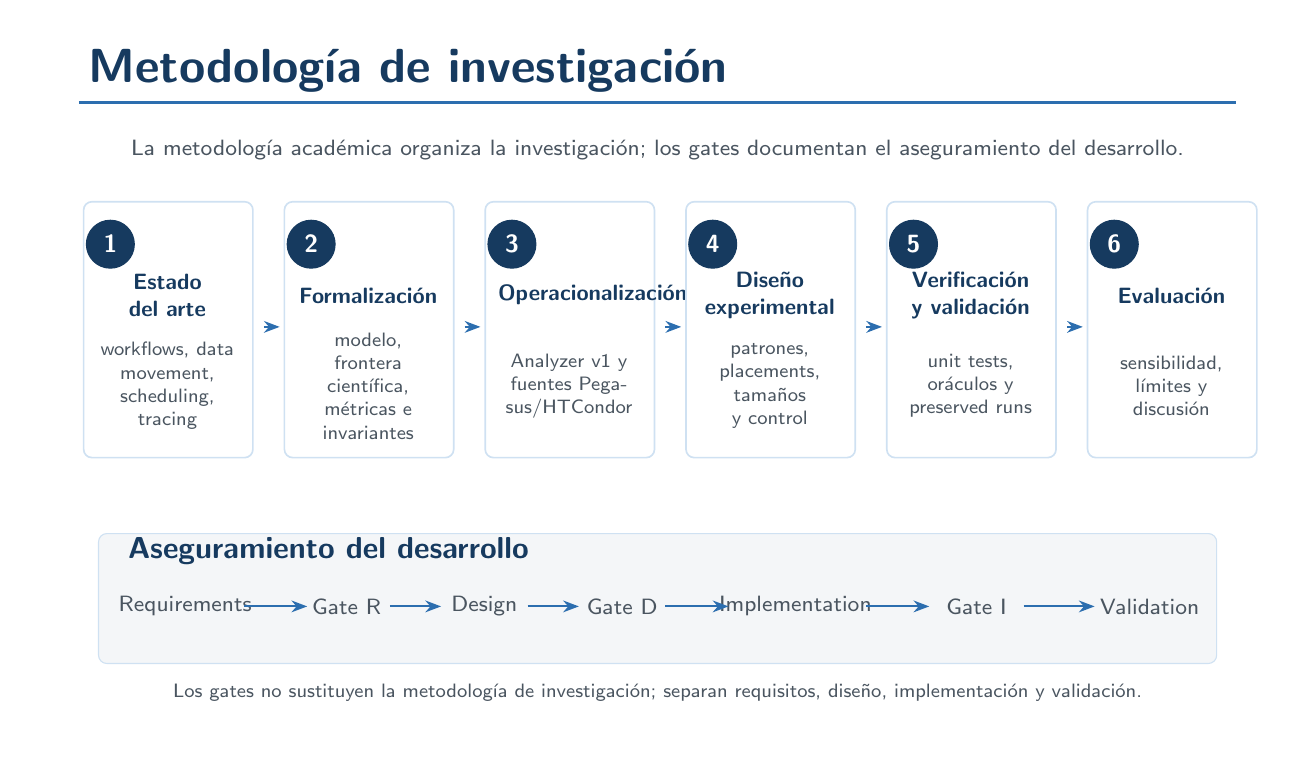
\begin{tikzpicture}[x=1cm,y=1cm]
\path[use as bounding box] (0,0) rectangle (16,9);
\node[title] at (0.65,8.45) {Metodología de investigación};
\draw[blue,line width=1pt] (0.65,8.05)--(15.35,8.05);
\node[small,text width=14.2cm,align=center] at (8,7.45) {La metodología académica organiza la investigación; los gates documentan el aseguramiento del desarrollo.};
\foreach \x/\n/\ttl/\sub in {
0.7/1/{Estado del arte}/{workflows, data movement, scheduling, tracing},
3.25/2/{Formalización}/{modelo, frontera científica, métricas e invariantes},
5.8/3/{Operacionalización}/{Analyzer v1 y fuentes Pegasus/HTCondor},
8.35/4/{Diseño experimental}/{patrones, placements, tamaños y control},
10.9/5/{Verificación y validación}/{unit tests, oráculos y preserved runs},
13.45/6/{Evaluación}/{sensibilidad, límites y discusión}}
{
\node[panel,minimum width=2.15cm,minimum height=3.25cm,anchor=north west] at (\x,6.8) {};
\node[draw=navy,fill=navy,circle,minimum size=0.5cm,font=\sffamily\bfseries\small,text=white] at (\x+0.35,6.25) {\n};
\node[font=\sffamily\bfseries\fontsize{8.5}{9.5}\selectfont,text=navy,text width=1.8cm,align=center] at (\x+1.075,5.6) {\ttl};
\node[tinylabel,text width=1.8cm,align=center] at (\x+1.075,4.45) {\sub};
}
\foreach \x in {3.0,5.55,8.1,10.65,13.2}{\draw[arrthin] (\x,5.2)--(\x+0.2,5.2);}
\node[rounded corners=3pt,draw=midblue,fill=lightgray,minimum width=14.2cm,minimum height=1.65cm] at (8,1.75) {};
\node[subtitle,anchor=west] at (1.15,2.35) {Aseguramiento del desarrollo};
\node[small,align=center] at (2.0,1.65) {Requirements}; \node[small,align=center] at (4.05,1.65) {Gate R}; \node[small,align=center] at (5.8,1.65) {Design}; \node[small,align=center] at (7.55,1.65) {Gate D}; \node[small,align=center] at (9.75,1.65) {Implementation}; \node[small,align=center] at (12.05,1.65) {Gate I}; \node[small,align=center] at (14.25,1.65) {Validation};
\draw[arrthin] (2.75,1.65)--(3.55,1.65); \draw[arrthin] (4.6,1.65)--(5.25,1.65); \draw[arrthin] (6.35,1.65)--(7.0,1.65); \draw[arrthin] (8.1,1.65)--(8.9,1.65); \draw[arrthin] (10.65,1.65)--(11.45,1.65); \draw[arrthin] (12.65,1.65)--(13.55,1.65);
\node[tinylabel,text width=13.4cm,align=center] at (8,0.55) {Los gates no sustituyen la metodología de investigación; separan requisitos, diseño, implementación y validación.};
\end{tikzpicture}
\end{document}
